%%% Preamble
\documentclass[paper=a4, fontsize=11pt]{scrartcl}	% Article class of KOMA-script with 11pt font and a4 format

\usepackage[english]{babel}															% English language/hyphenation
\usepackage[protrusion=true,expansion=true]{microtype}				% Better typography
\usepackage{amsmath,amsfonts,amsthm}										% Math packages
\usepackage[pdftex]{graphicx}														% Enable pdflatex
%\usepackage{color,transparent}													% If you use color and/or transparency
\usepackage[hang, small,labelfont=bf,up,textfont=it,up]{caption}	% Custom captions under/above floats
\usepackage{epstopdf}																	% Converts .eps to .pdf
\usepackage{subfig}																		% Subfigures
\usepackage{booktabs}																	% Nicer tables
\usepackage{graphicx}
\graphicspath{ {images/} }

%%% Advanced verbatim environment
\usepackage{verbatim}
\usepackage{fancyvrb}
\DefineShortVerb{\|}								% delimiter to display inline verbatim text


%%% Custom sectioning (sectsty package)
\usepackage{sectsty}								% Custom sectioning (see below)
\allsectionsfont{%									% Change font of al section commands
	\usefont{OT1}{bch}{b}{n}%					% bch-b-n: CharterBT-Bold font
%	\hspace{15pt}%									% Uncomment for indentation
	}

\sectionfont{%										% Change font of \section command
	\usefont{OT1}{bch}{b}{n}%					% bch-b-n: CharterBT-Bold font
	\sectionrule{0pt}{0pt}{-5pt}{0.8pt}%	% Horizontal rule below section
	}


%%% Custom headers/footers (fancyhdr package)
\usepackage{fancyhdr}
\pagestyle{fancyplain}
\fancyhead{}														% No page header
\fancyfoot[C]{\thepage}										% Pagenumbering at center of footer
\fancyfoot[R]{\small \texttt{Victor Frolov}}	% You can remove/edit this line 
\renewcommand{\headrulewidth}{0pt}				% Remove header underlines
\renewcommand{\footrulewidth}{0pt}				% Remove footer underlines
\setlength{\headheight}{13.6pt}

%%% Equation and float numbering
\numberwithin{equation}{section}															% Equationnumbering: section.eq#
\numberwithin{figure}{section}																% Figurenumbering: section.fig#
\numberwithin{table}{section}																% Tablenumbering: section.tab#


%%% Title	
\title{ \vspace{-1in} 	\usefont{OT1}{bch}{b}{n}
		\huge \strut Battle of the Wearables and Their Interaction Designs \strut \\
		\Large \bfseries \strut Comparing the Apple Watch to Google Glass \strut
}
\author{ 									\usefont{OT1}{bch}{m}{n}
        Victor Frolov\\		\usefont{OT1}{bch}{m}{n}
        Loyola Marymount University\\	\usefont{OT1}{bch}{m}{n}
	Assignment 0924\\
}
\date{September 24, 2015}

%%% Begin document
\begin{document}
\maketitle
\section{Introduction}
	Wearable technology is becoming mainstream and is ranging from products such as fitness trackers, accessories to phones and even glasses that display information and allow you a virtual reality HUD. This report will attempt to objectively declare a superior user experience through interaction design from two infamous competing companies: Google and Apple.

	Below are two sections; the first provides usability measures and a conclusion on which device performed better, and the second dives into why this was the case. The usability of the  Apple Watch versus Google Glass will be measured with the following three tasks: 

\begin{itemize}
	\item Have the user send the following text message to any contact: ``I'm sorry Dave, I'm afraid I can't do that."
	\item Have the user set driving directions from Loyola Marymount University to Staples Center.
	\item Have the user set  a reminder for October 10th, 2017, with the title "Thanks Obama"
\end{itemize}

The measurable usabilities will fall under the following three categories: Learnability, Errors and Satisfaction.


\section{Usability Measures}
\subsection{Task One: Sending a text message}
The user must send the following text message to the contact \textit{Aleksandar Frolov} : ``I'm sorry Dave, I'm afraid I can't do that.''


\subsubsection{Learnability}

Users were timed, demonstrating how long it would take someone who has never used the device to complete a task. Each bar represents a user, and the height represents how many seconds it took to complete the task. It is obvious that the Apple Watch's learnability beat out Google Glass.

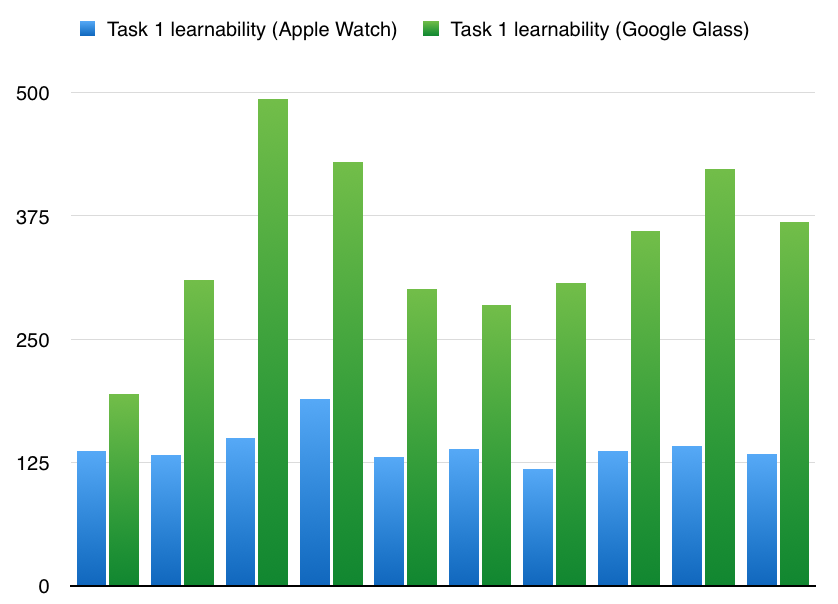
\includegraphics[scale=0.7]{charttask1}

Below is the average time for a user to complete a task, in seconds. Green bar's height represents the average time to complete the task using Google Glass in seconds, and the blue bar represents the average time to complete the task in seconds using the Apple Watch.

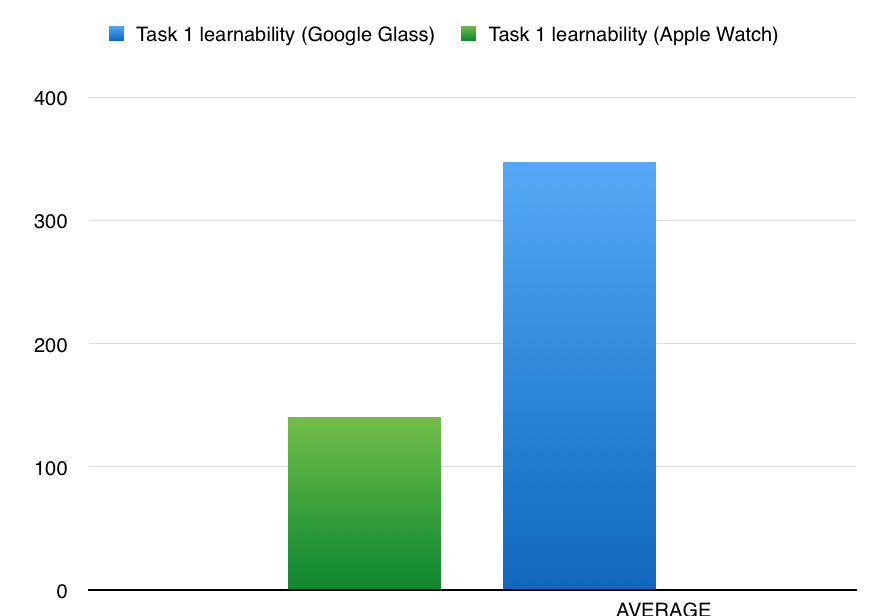
\includegraphics[scale=0.6]{task1average}

The Apple Watch's Average time to complete the task was 140.4 seconds, whereas Google Glass took 347, which was almost 2.5 times slower.


\subsubsection{Errors}
User errors were tracked when attempting to send a text message.

\textbf{Apple Watch}
4 out of 10 users assumed that pressing on crown would open keyboard and returned to the home screen instead. The same 4 users  shut off the screen by pressing lock button right after.
3 out of 10 users had voice recognition issues, which  may have been due to slurring of the words.
1 user was stuck in the watch face, confused how to exit it.


\textbf{Google Watch}
10 out of 10 users mistapped or swiped incorrectly causing the user to return back to the menu. 
6 out of 10 users had voice recognition issues, where the message would cut out early. Could be due to slurring of the words.


\subsubsection{Satisfaction}
Below is the user overall satisfaction when attempting to send the text message.

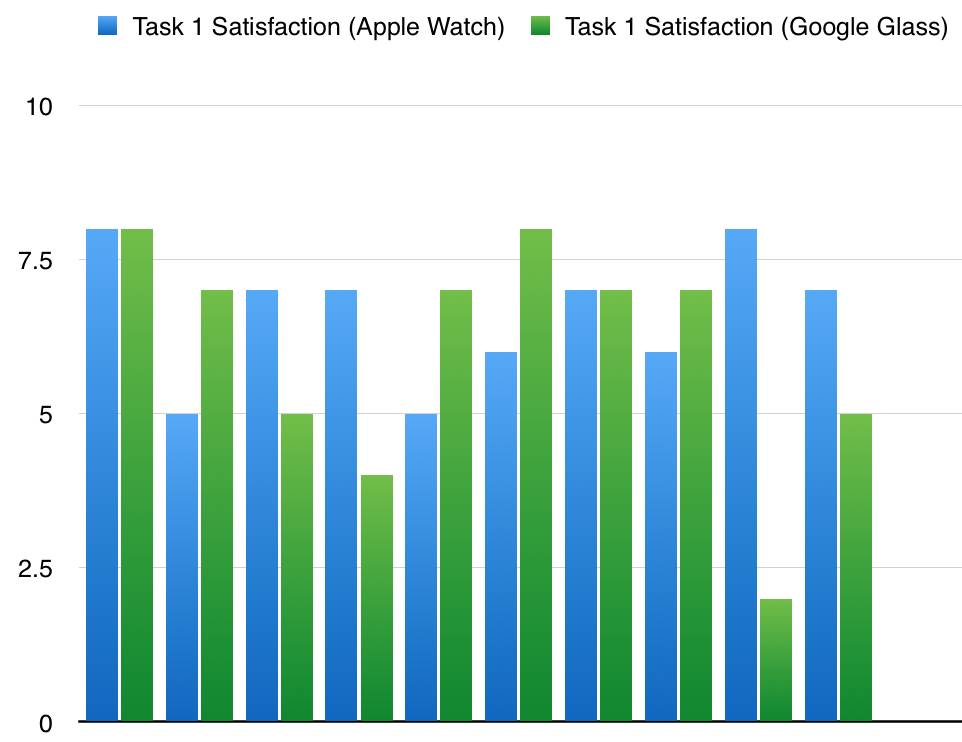
\includegraphics[scale=0.8]{task1satisfaction}\\ \\

Below is the average satisfaction (blue represents Apple Watch, green represents Google Glass)\\ \\

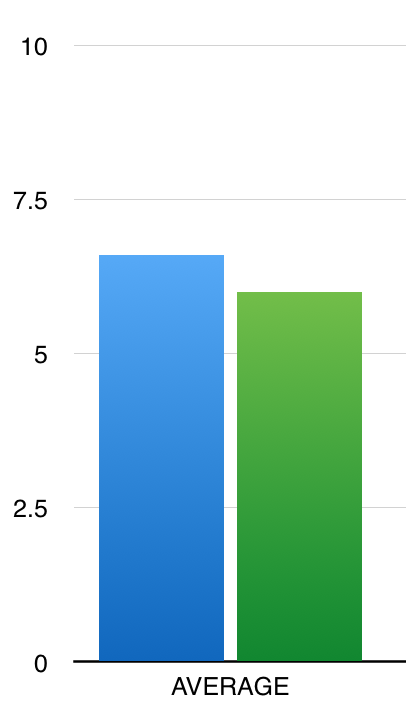
\includegraphics[scale=0.8]{task1satav}



Remarkably, even though each user struggled using Google Glass, and ran into far more errors, and took much longer on average to send a text message(with the only outlier being a quick completion) the subjective satisfaction was very close, landing at 6.6/10 for the Apple Watch, and 6/10 for Google Glass

\subsection{Task Two: Set Driving Directions}
Have the user set driving directions from Loyola Marymount University to Staples Center.

\subsubsection{Learnability}
Users were timed, demonstrating how long it would take someone who has never used the device to complete a task. Each bar represents a user, and the height represents how many seconds it took to complete the task. It is obvious that the Apple Watch's learnability beat out Google Glass.

Below is a chart for time taken to complete the task (each bar represents a user, and the time on the y axis is in seconds)

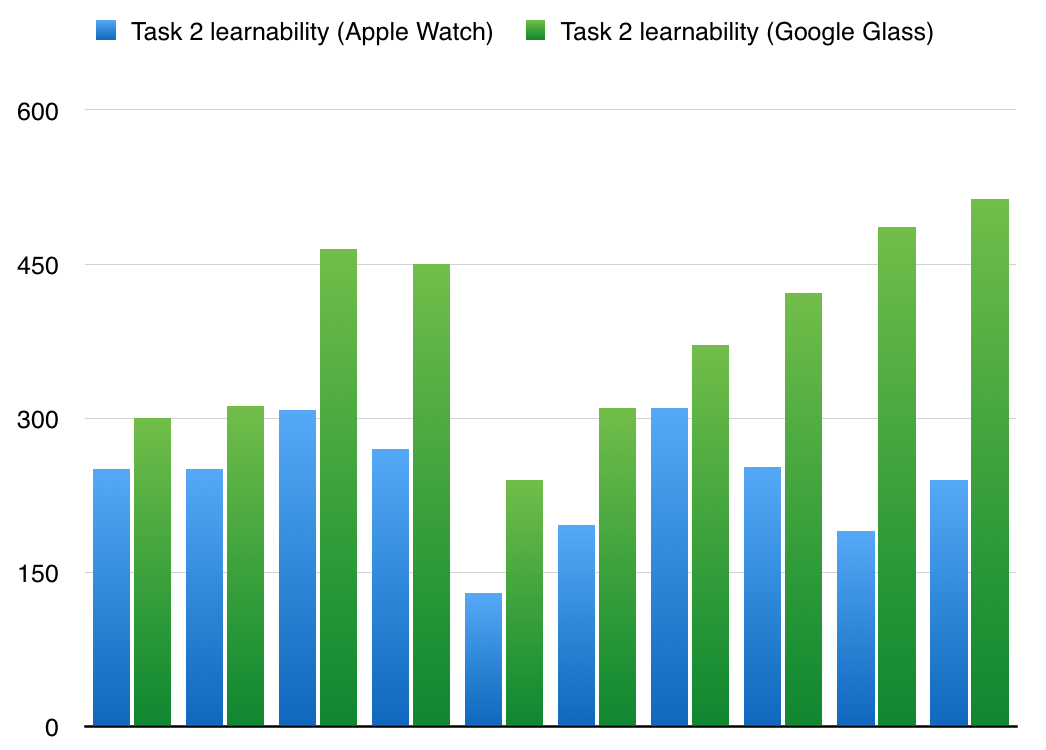
\includegraphics[scale=0.8]{task2learnability}


Below is a chart for time taken to complete the task on average, where the y axis is in seconds.

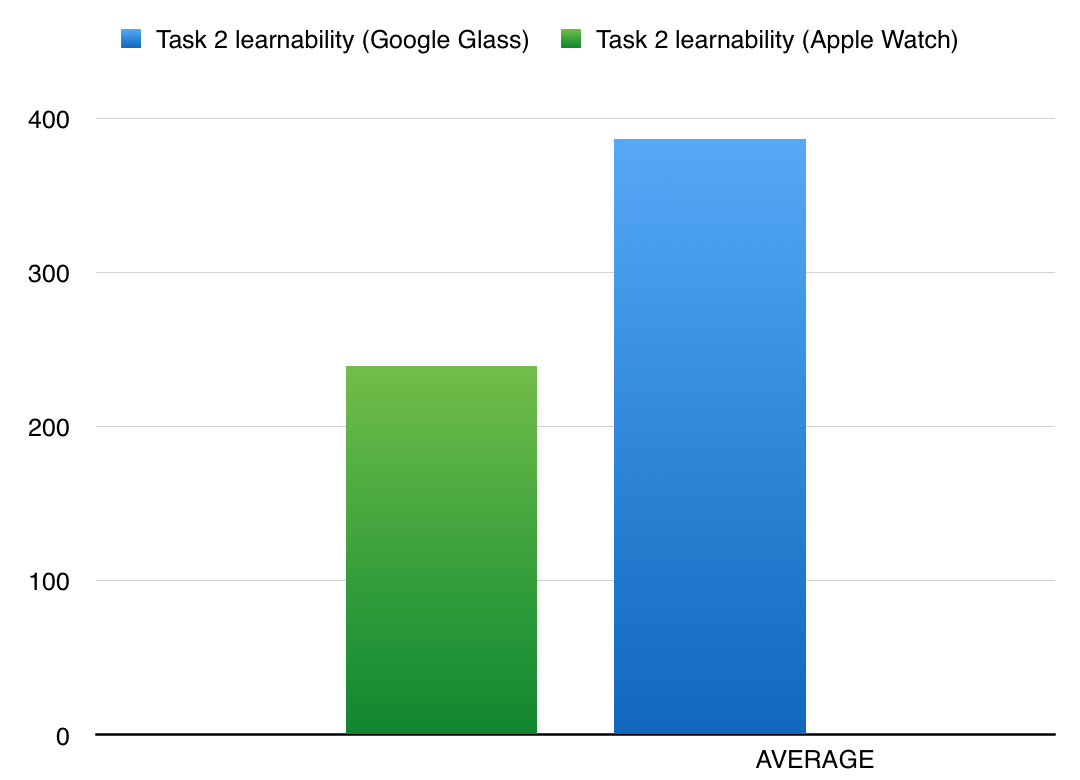
\includegraphics[scale=0.6]{task2learnav}

On average, users were 1.6 times faster on the Apple Watch than they were on Google Glass. Comparing to task 1, this is much closer.

\subsubsection{Errors}

User errors were tracked when attempting to navigate.\\

\textbf{Apple Watch} \\
9 out of 10 users pressed on crown assuming it would drop a pin. 4/10 attempted pinch to zoom functionality, and were unsucessful.

\textbf{Google Watch}\\
4 out of 10 users mistapped causing the app to quit. 3 out of 10 users were impatient and continued to tap on the touch pad due to map loading slowly. 5 out of 10 users found it unintuitive to drop a pin, and found that the most difficult part (while located at LMU). 2 out of 10 users got directions to Staples instead of the Staples Center.


\subsubsection{Satisfaction}
Below is the user overall satisfaction when attempting to find directions.

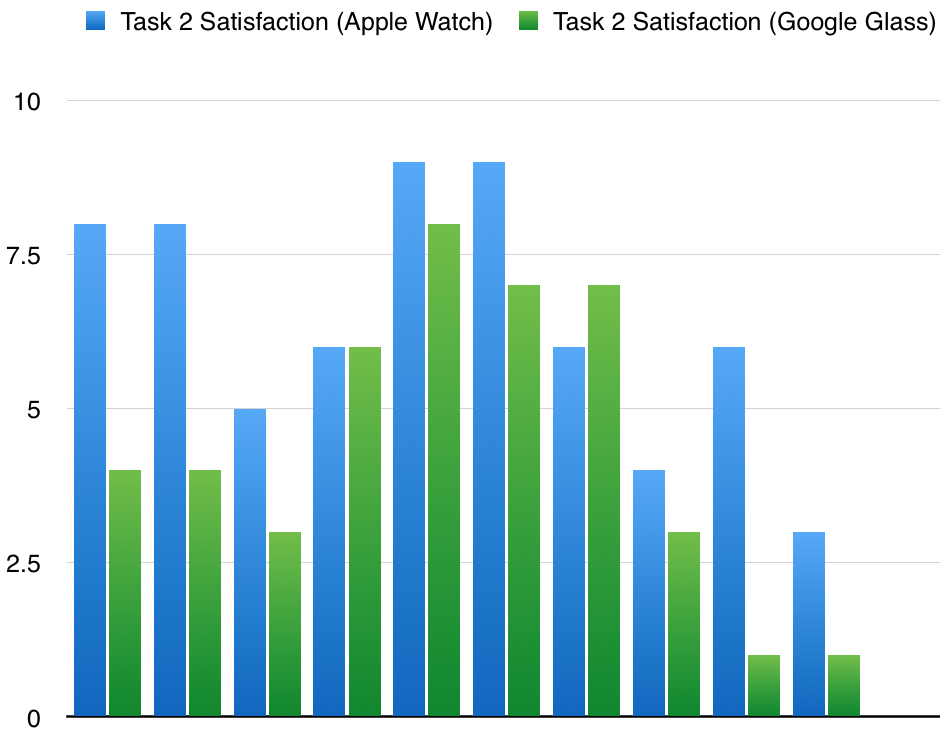
\includegraphics[scale=0.8]{task2sat}\\ \\

Below is the average satisfaction (blue represents Apple Watch, green represents Google Glass)\\ \\

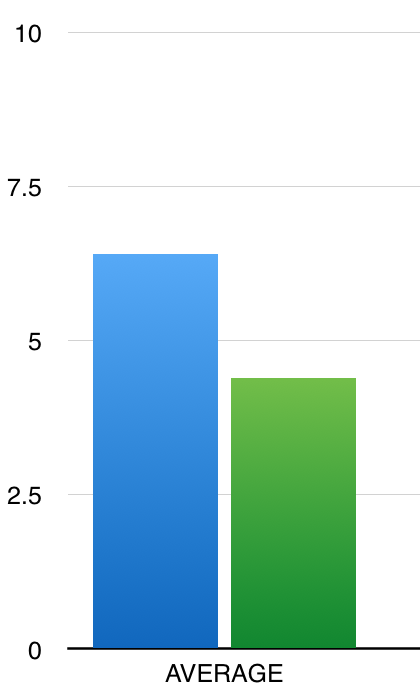
\includegraphics[scale=0.8]{task2satav}

Average for satisfaction for the Apple Watch and Google Glass were 6.4/10 and 4.4/10 respectively. Albeit being relatively close, the Google Glass got very unfavorable reviews, only one user graded satisfaction above a 7, while three users satisfaction above a 7 for Apple Watch.

\subsection{Task Three: Set Reminder}
Have the user set  a reminder for October 10th, 2017, with the title "Thanks Obama"

\subsubsection{Learnability}
Users were timed, demonstrating how long it would take someone who has never used the device to complete a task. Each bar represents a user, and the height represents how many seconds it took to complete the task. 

Below is a chart for time taken to complete the task (each bar represents a user, and the time on the y axis is in seconds)

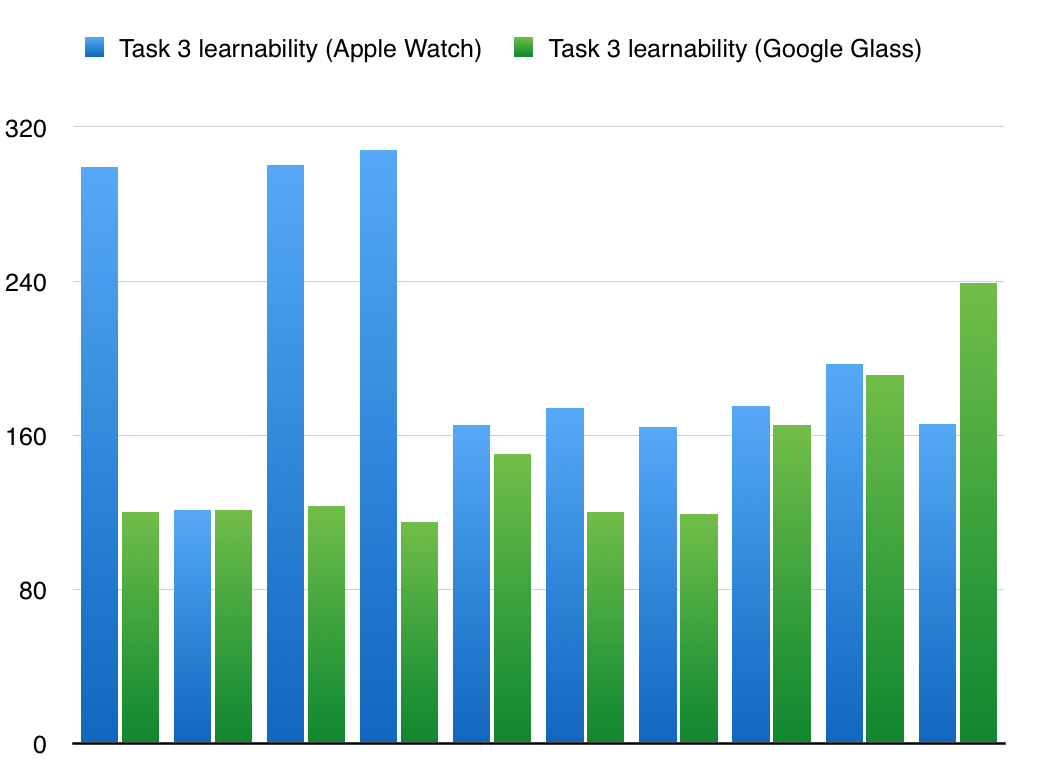
\includegraphics[scale=0.8]{task3learnability}


Below is a chart for time taken to complete the task on average, where the y axis is in seconds.

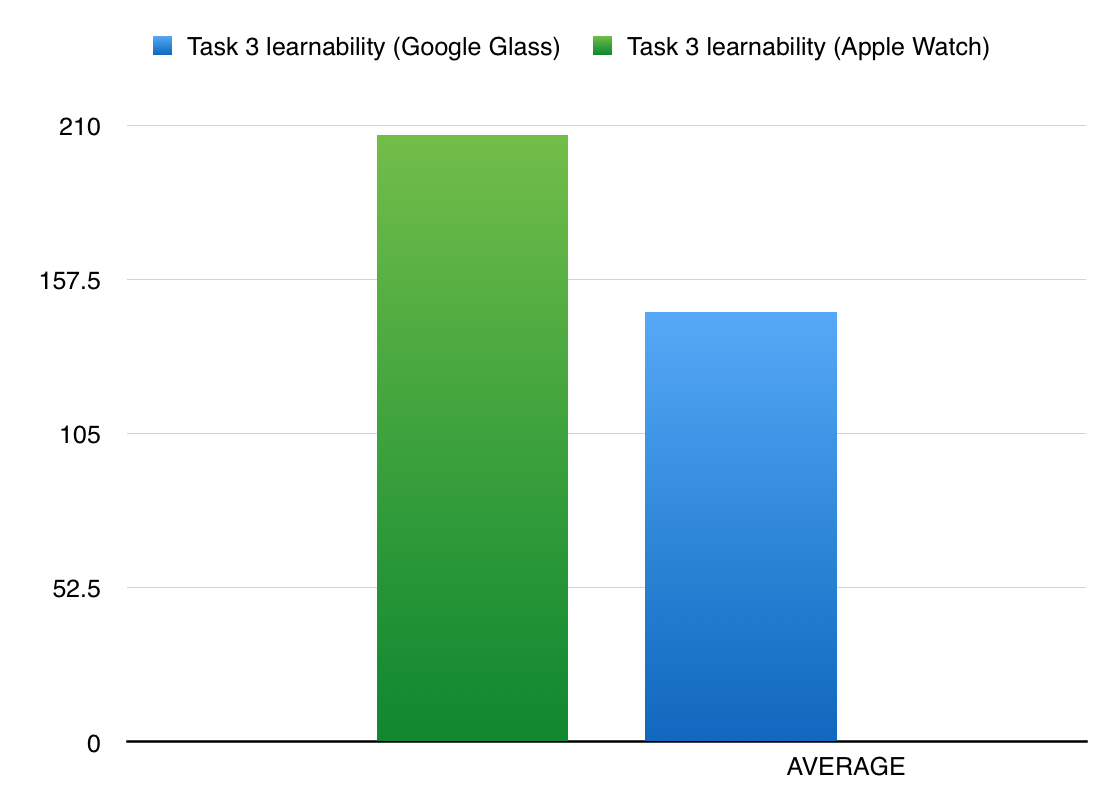
\includegraphics[scale=0.6]{task3learnav}

On average users were 1.4 times faster in completing the reminders task on Google Glass over Apple Watch, with 206.9 seconds average for the watch, and 146.3 seconds average for the glasses. This is the only one of the three tasks where users completed a task faster on Google Glass than on the Apple Watch.


\subsubsection{Errors}
User errors were tracked when attempting to set a reminder.\\

\textbf{Apple Watch} \\
2 out of 10 users accidentally quit the application, having to restart from scratch(action to quit application was not provided by tester). 3 out10 users encountered voice command issues, could be slurring of the words. 3 out of 10 users put the incorrect date having to restart from scratch.
 
\textbf{Google Watch}\\
Remarkably, there were no errors for any users.

\subsubsection{Satisfaction}
Below is the user overall satisfaction when attempting to set a reminder.

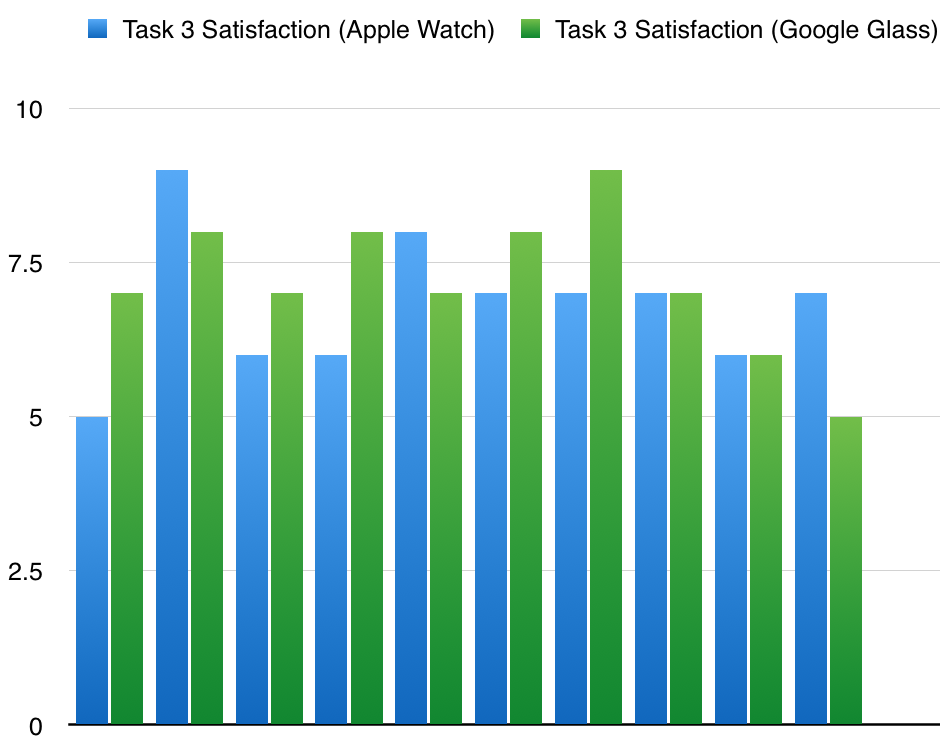
\includegraphics[scale=0.8]{task3sat}\\ \\

Below is the average satisfaction (blue represents Apple Watch, green represents Google Glass)\\ \\

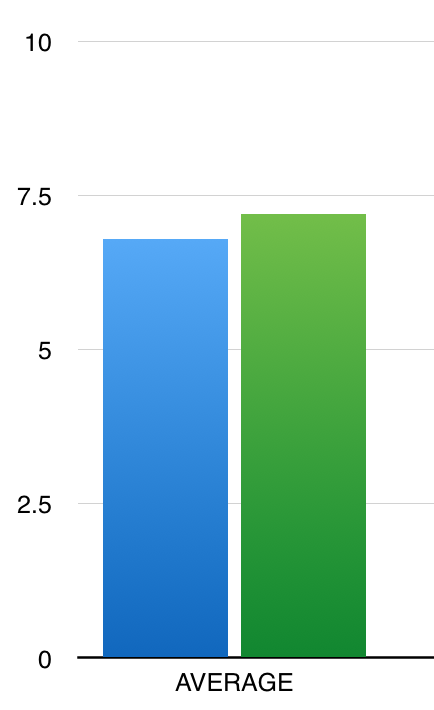
\includegraphics[scale=0.8]{task3satav}

Average for satisfaction for the Apple Watch and Google Glass were 6.8/10 and 7.2/10 respectively. Albeit the Apple Watch taking considerably longer (1 min), the user experience was almost identical.




\subsubsection{Conclusion}
Deciding on which of the two wearables has better interaction design is a hard question to answer. There are many factors to take into consideration. For example, people are relatively familiar with touch screens, and the apple watch is simply a smaller touch screen with force touch, but a product like Google Glass is something most people have never experienced. Another consideration to have is the Apple Watch being a finalized product sold to end users, whereas Google Glass was still under beta prior to it being shut down.  

Regardless, we have measurable statistics above to come to a conclusion, so to summarize, the Apple watch was considerably faster to accomplish all three tasks, averaging at 199 seconds, whereas Google Glass averaged at 291. User errors were all over the place, but all 10 out of 10 users mistapped on Google Glass in the first task. User satisfaction averaged a 6.6 for the Apple Watch, and 5.9 for Google Glass, so it appears that the Apple Watch performed better. 



\section{Mathematics}
Let's display some math:
\begin{align} 
	\begin{split}
	(x+y)^3 	&= (x+y)^2(x+y)\\
					&=(x^2+2xy+y^2)(x+y)\\
					&=(x^3+2x^2y+xy^2) + (x^2y+2xy^2+y^3)\\
					&=x^3+3x^2y+3xy^2+y^3
	\end{split}					
\end{align}

\begin{align}
	A = 
	\begin{bmatrix}
	A_{11} & A_{21} \\
  	A_{21} & A_{22}
	\end{bmatrix}
\end{align}

\end{document}